\section{Exploratory Testing}
\label{sec:Exploratory Testing}

\rindex{\textbf{E}!Exploratory Testing}A very cool, but informal test design technique.

It is hard to explain this approach in a few words, because it is completely unusual for almost all testers. But it can be demonstrated and explained step-by-step (it's like riding a bicycle).

Here is the simplest explanation of this approach:

\begin{figure}[!h]
\centering
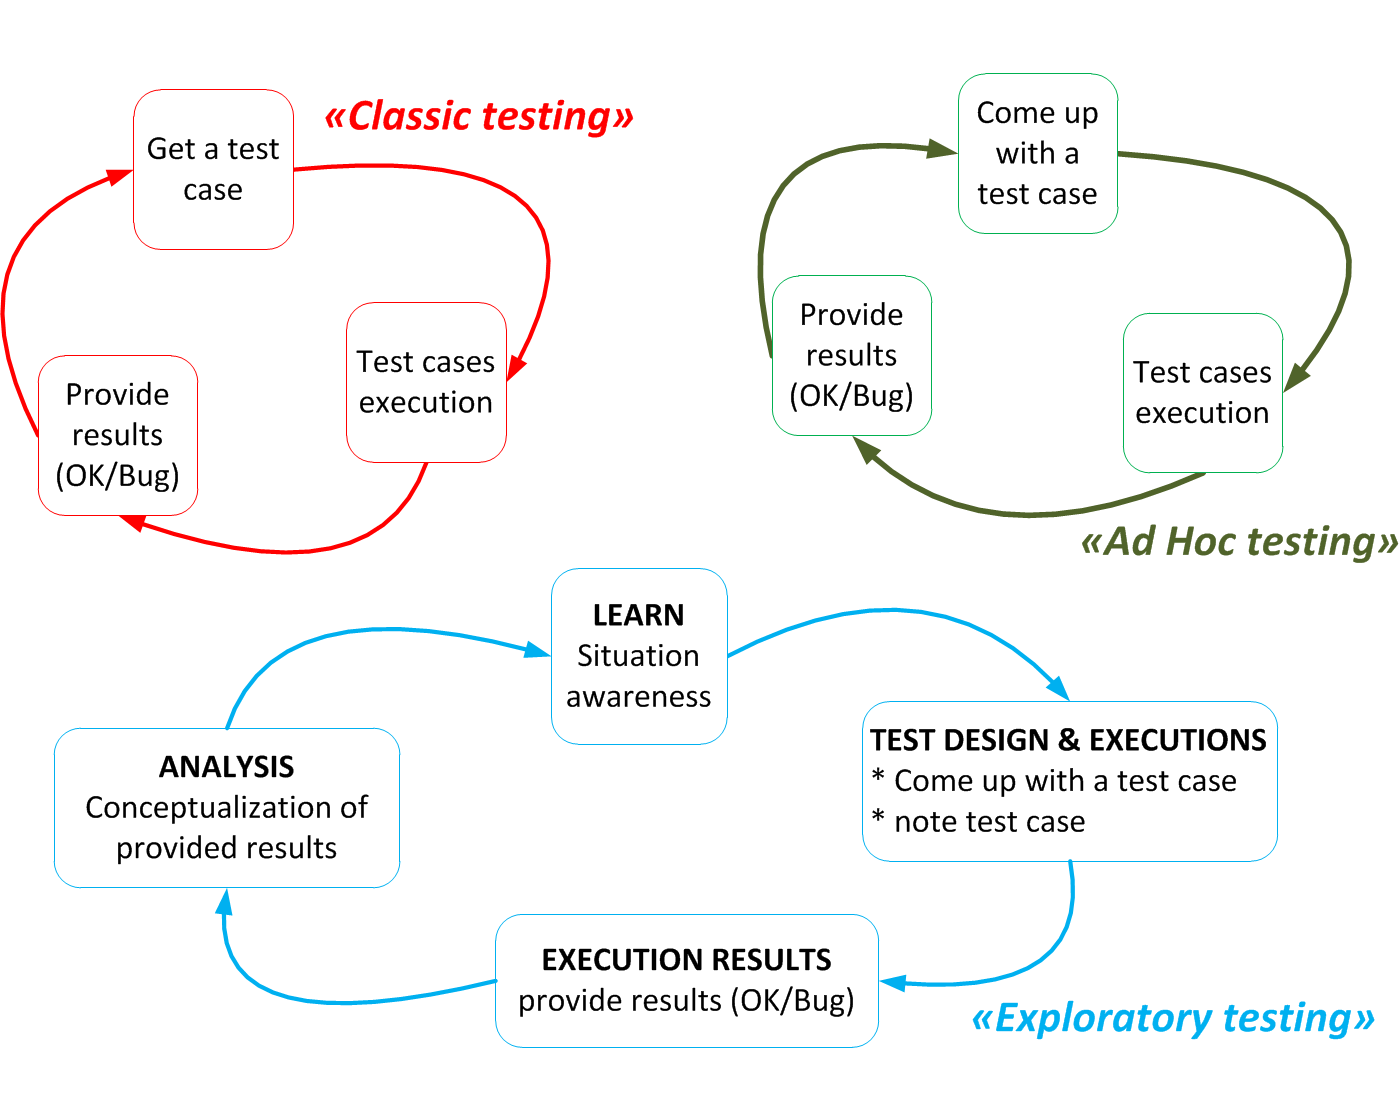
\includegraphics[width=\linewidth]{ClassicAdHocExploratoryTesting}
\caption{\ttfamily{Simple explanation of Classic \& Ad Hoc \& Exploratory testing}}
\label{fig:ClassicAdHocExploratoryTesting}
\end{figure}
